% fluxograma_metodologia_nm.tex
\documentclass[border=8pt]{standalone}
\usepackage{tikz}
\usetikzlibrary{shapes.geometric, arrows.meta, positioning, calc}

\begin{document}
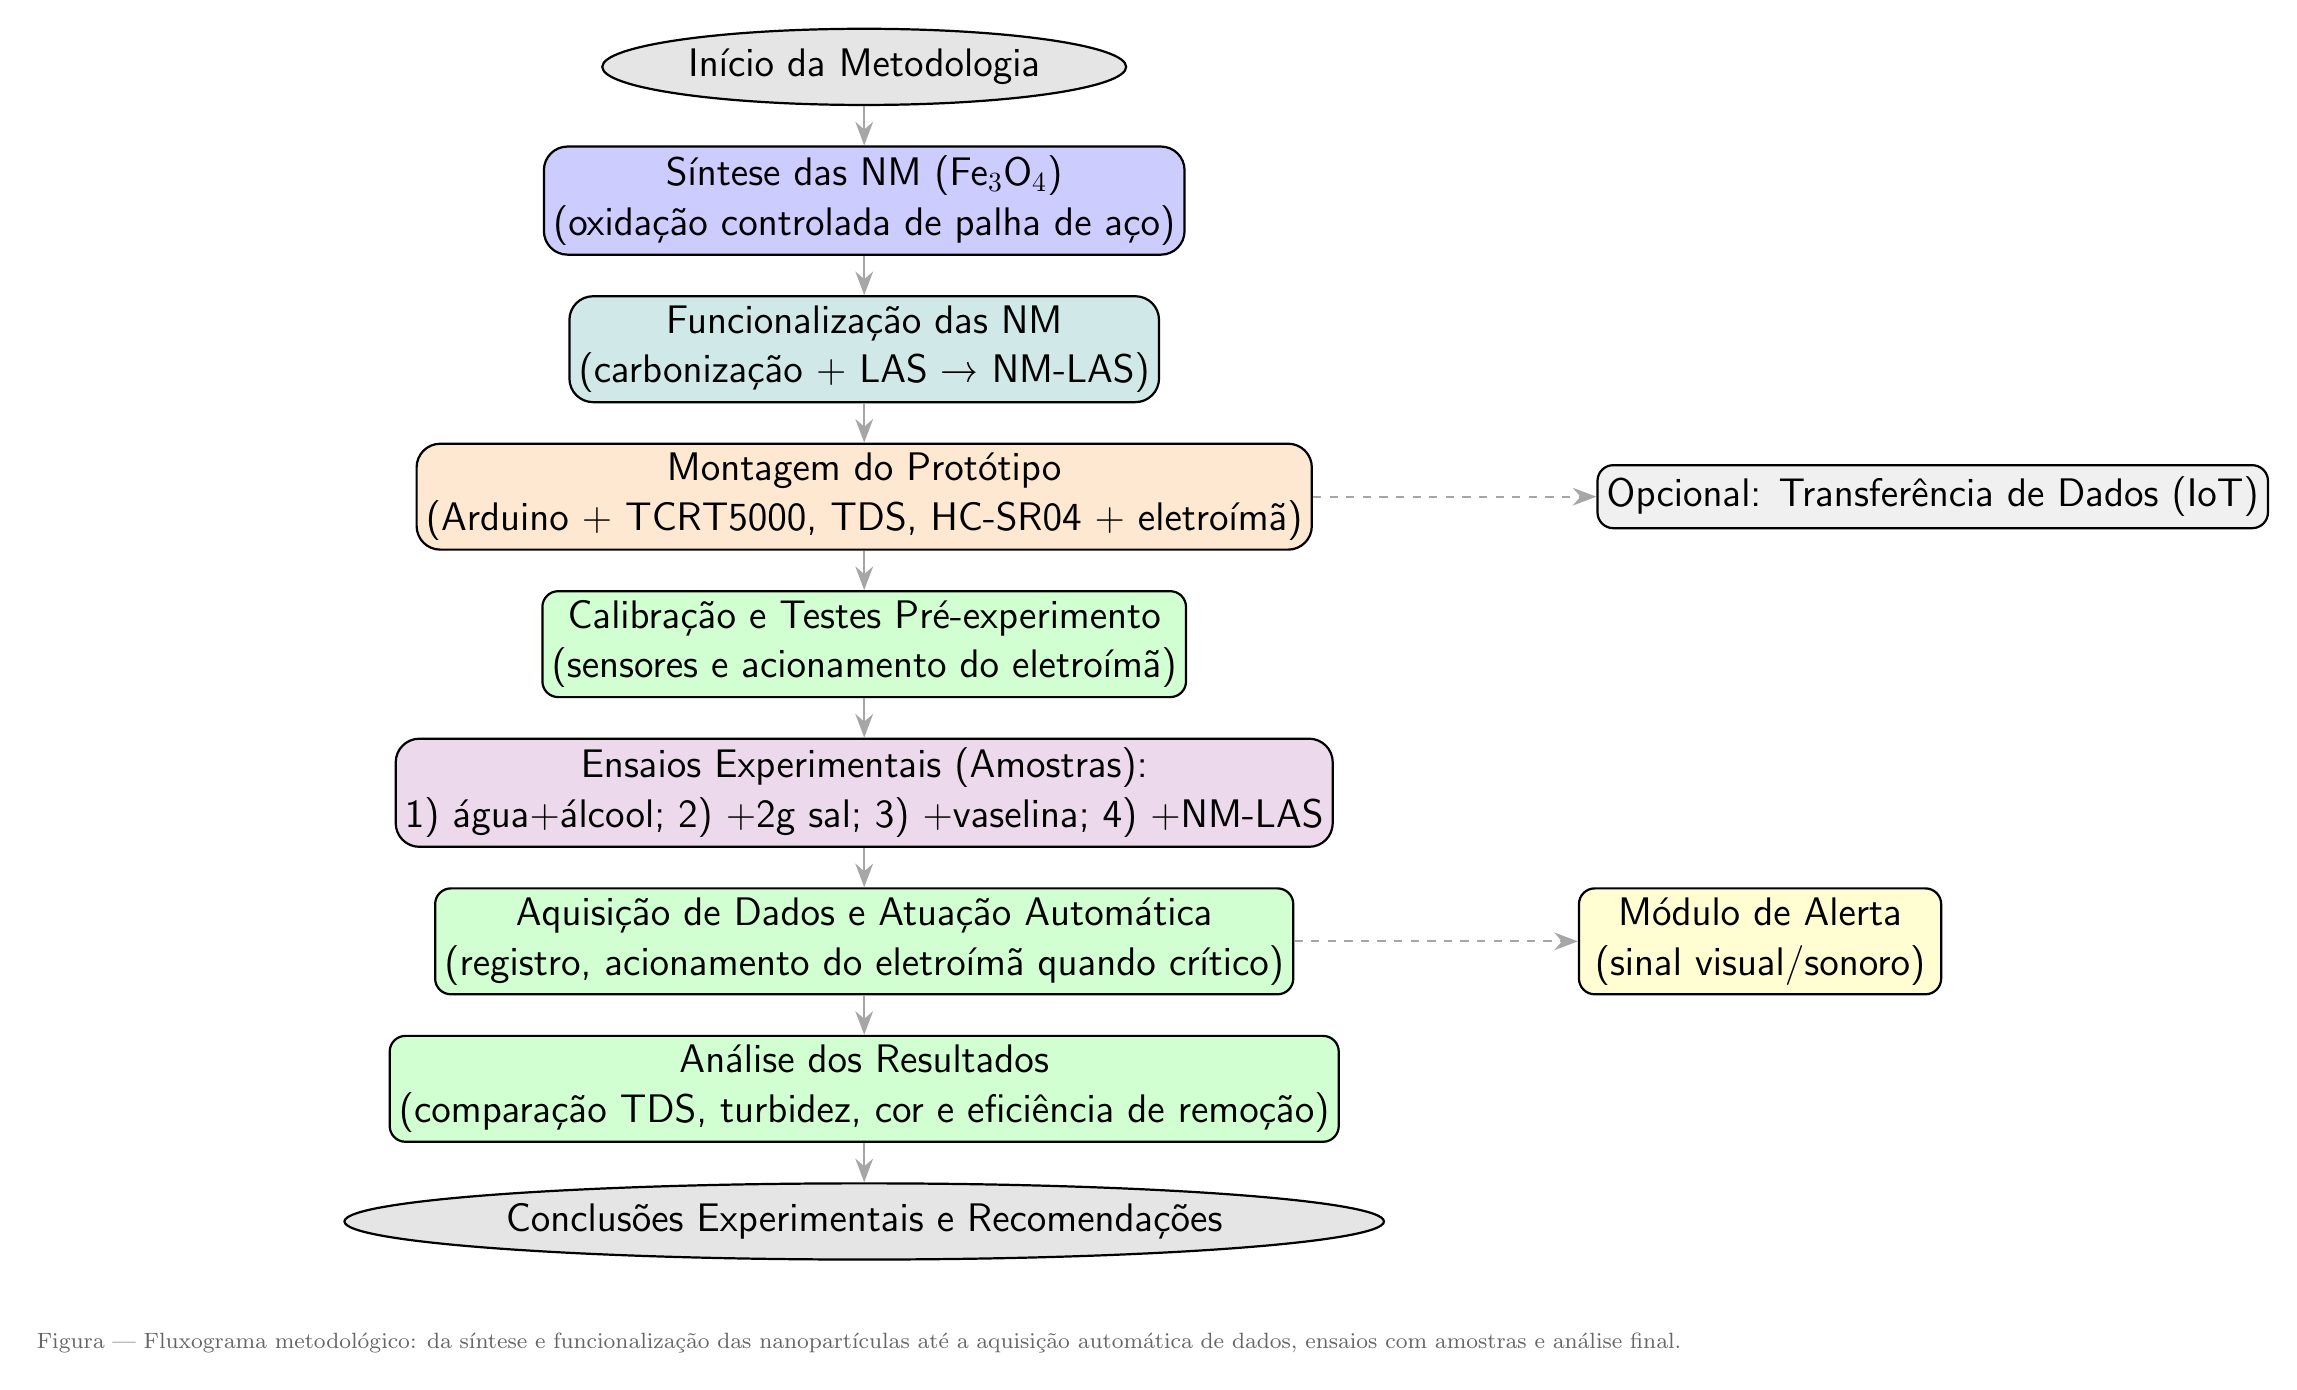
\begin{tikzpicture}[
  node distance=5mm and 10mm,
  font=\sffamily\Large,
  startstop/.style={ellipse, draw, thick, fill=gray!20, minimum width=40mm, minimum height=9mm, align=center},
  stepA/.style={rectangle, rounded corners=3mm, draw, thick, fill=blue!20, minimum width=56mm, minimum height=10mm, align=center},
  stepB/.style={rectangle, rounded corners=3mm, draw, thick, fill=teal!18, minimum width=56mm, minimum height=10mm, align=center},
  stepC/.style={rectangle, rounded corners=3mm, draw, thick, fill=orange!18, minimum width=66mm, minimum height=10mm, align=center},
  stepD/.style={rectangle, rounded corners=3mm, draw, thick, fill=violet!15, minimum width=66mm, minimum height=10mm, align=center},
  process/.style={rectangle, rounded corners=2mm, draw, thick, fill=green!18, minimum width=58mm, minimum height=9mm, align=center},
  arrow/.style={thick, -{Stealth[length=3mm]}, gray!70},
  dashedarrow/.style={thick, -{Stealth[length=3mm]}, gray!70, dashed}
]

% Nodes (vertical main flow)
\node[startstop] (inicio) {Início da Metodologia};
\node[stepA, below=of inicio] (sint) {Síntese das NM (Fe$_3$O$_4$)\\(oxidação controlada de palha de aço)};
\node[stepB, below=of sint] (func) {Funcionalização das NM \\(carbonização + LAS → NM-LAS)};
\node[stepC, below=of func] (mont) {Montagem do Protótipo\\(Arduino + TCRT5000, TDS, HC-SR04 + eletroímã)};
\node[process, below=of mont] (calib) {Calibração e Testes Pré-experimento \\(sensores e acionamento do eletroímã)};
\node[stepD, below=of calib] (teste) {Ensaios Experimentais (Amostras):\\1) água+álcool; 2) +2g sal; 3) +vaselina; 4) +NM-LAS};
\node[process, below=of teste] (daq) {Aquisição de Dados e Atuação Automática\\(registro, acionamento do eletroímã quando crítico)};
\node[process, below=of daq] (analise) {Análise dos Resultados \\(comparação TDS, turbidez, cor e eficiência de remoção)};
\node[startstop, below=of analise] (fim) {Conclusões Experimentais e Recomendações};

% Arrows main flow
\draw[arrow] (inicio) -- (sint);
\draw[arrow] (sint) -- (func);
\draw[arrow] (func) -- (mont);
\draw[arrow] (mont) -- (calib);
\draw[arrow] (calib) -- (teste);
\draw[arrow] (teste) -- (daq);
\draw[arrow] (daq) -- (analise);
\draw[arrow] (analise) -- (fim);

% Side modules: Alerta e IoT (dashed)
\node[rectangle, rounded corners=2mm, draw, thick, fill=yellow!18, minimum width=46mm, minimum height=8mm, align=center, right=36mm of daq] (alert) {Módulo de Alerta \\(sinal visual/sonoro)};
\node[rectangle, rounded corners=2mm, draw, thick, fill=gray!12, minimum width=46mm, minimum height=8mm, align=center, right=36mm of mont] (iot) {Opcional: Transferência de Dados (IoT)};

\draw[dashedarrow] (daq.east) -- (alert.west);
\draw[dashedarrow] (mont.east) -- (iot.west);

% Annotation / caption
\node[below=8mm of fim, font=\footnotesize, align=center, color=black!60] {
Figura — Fluxograma metodológico: da síntese e funcionalização das nanopartículas até a aquisição automática de dados, ensaios com amostras e análise final.
};

\end{tikzpicture}
\end{document}

